\section{\change{The Effect of Heavy Rainfall Clustering on Clouds and Humidity}{Heavy Rainfall Clustering and Radiative feedbacks associated with Climate Sensitivity}}
We now consider how large-scale clustering of precipitation influences the cloud and humidity distribution. 
Our motivation is to understand how such clustering may \change[\firstAuthorEdit]{influence}{connect to} radiative feedbacks. 
Previous authors have found that the degree of clustering on different spatial scales 
has an effect on the radiation budget and clouds \citep[e.g.,][]{Bony2020, wing2014, Pendergrass2016}. 
The literature suggests changes in clustering under warming may lead to 
different cloud feedbacks and may therefore affect equilibrium climate sensitivity (ECS) \citep{Schiro2022}. 
This section investigates this hypothesis for large-scale clustering across the CMIP6 ensemble. 
As for previous sections, the analysis assesses whether relationships in interannual variability can be used to infer the response to climate change, 
raising the possibility of an observational constraint on particular radiative feedbacks or ECS itself. 

Rather than focusing on changes in radiative fluxes or calculating feedback strength directly, 
we focus on changes in mid-tropospheric relative humidity, 
which has been argued to cause a negative longwave feedback associated with changes in convective organization \citep{Tobin2013,Bony2020}, 
and changes in low-cloud fraction in regions of subsidence, 
which have been argued to cause a positive shortwave feedback associated with changes in convective organization \citep{Schiro2022}. 
Changes in low clouds in regions of subsidence are also known to be important for understanding model spread in ECS \citep{Zelinka2020}. 
Correlations between measures of large-scale clustering of heavy precipitation and various other metrics commonly used to assess changes to the radiation budget on 
interannual and climatological timescales are presented in Figure S1-\change[\firstAuthorEdit]{4}{2} in the supporting information.

For our analysis, the mid-tropospheric relative humidity, RH, is taken as the 500 hPa value, 
\remove[\firstAuthorEdit]{but the conclusions are not sensitive to using proximate pressure levels down to 700 hPa.}
Observed low-cloud fraction, LCF, is calculated using the ISCCP weather states \citep{Tselioudis2010} as described in Section \ref{sec:methods:obs}, 
and taken as the cloud fraction below 600 hPa. CMIP6 low-cloud fraction is calculated analogously, 
with cloud fraction pre-processed by interpolating hybrid-sigma coordinates to 19 pressure levels if not already available on pressure levels. 
We also consider the mean low-cloud fraction in regions of descent, denoted by a subscript $d$ 
and calculated as the \add[\firstAuthorEdit]{tropical-}mean of gridpoints for which the monthly-mean vertical pressure velocity at 500 hPa is positive. 
Later we will consider variables in regions of ascent, defined analogously for negative 500 hPa vertical velocity and identified by a subscript $a$.

Figure \ref{radiation_obsMAP_BOX_RH}a and Figure \ref{radiation_obsMAP_BOX_LCF}a show observational estimates of the regression patterns of RH and LCF 
against the mean area of precipitation features, $A_m$, for interannual variability. 
The regressions show a clear El-Ni\~no-like pattern, with increases in RH and decreases in LCF in the central and eastern Pacific, 
and opposite changes over the warm pool. This suggests the changes in RH and low clouds with increased tropical clustering are caused at least in part 
by variations associated with El Ni\~no-Southern Oscillation.

From a tropics-wide perspective, when the observed degree of clustering is high according to $A_m$, the tropical mean is drier (Figure \ref{radiation_obsMAP_BOX_RH}b) 
while LCF increases, both when averaged over descending grid points (LCF$_d$ in Figure \ref{radiation_obsMAP_BOX_LCF}b) 
and in regions of time-mean descent (contour on Figure \ref{radiation_obsMAP_BOX_LCF}a). 
The environmental signature associated with large-scale clustering is therefore consistent with a negative longwave feedback 
identified for large-scale clustering in idealized simulations \citep{Arnold2015} and a longwave- and low-cloud cooling signature found associated with 
interannual variations in mesoscale organization in observations \citep{Bony2020}. 
However, partial correlations of $A_m$ with RH excluding the influence of the total area 
\change[\firstAuthorEdit]{
fraction of heavy precipitation, $A_f$, 
}{
coverage of heavy precipitation, $C$,
}
are insignificant in the observations (Figure \ref{radiation_obsMAP_BOX_RH}b). 
This suggests that the influence of $A_m$ on relative humidity is almost entirely due to increasing \change[\firstAuthorEdit]{$A_f$}{$C$}. 
Observed correlations of relative humidity and the distance metrics \change[\firstAuthorEdit]{$C_m$}{$P_{eq}$, $P_{heq}$} and \change[\firstAuthorEdit]{$C_z$}{$P_{z}$}, 
representing proximity of heavy rainfall to the equator and the central Pacific, respectively, are also generally insignificant. 
Observed LCF$_d$ on the other hand increases for all three forms of spatial clustering, outside the influence of \change[\firstAuthorEdit]{$A_f$}{$C$} 
(Figure \ref{radiation_obsMAP_BOX_LCF}b).

The CMIP6 ensemble generally agrees on the strong association between \change[\firstAuthorEdit]{$A_f$}{$C$} and the aforementioned tropical environmental signatures. 
However, unlike the observational estimates, about half of the models also show a significant relationship between relative humidity 
and spatial shifts of heavy precipitation (Figure \ref{radiation_obsMAP_BOX_RH}b). In particular, in a subset of models, 
zonal shifts in heavy precipitation to the central Pacific are (independent of variations in \change[\firstAuthorEdit]{$A_f$}{$C$}) associated with a moistening in the tropics, 
while meridional shifts to the equator result in domain-mean drying. These relationships are also present in the high-resolution GCM. 
The models generally do not capture the observed LCF$_d$ signature for clustering outside the influence of \change[\firstAuthorEdit]{$A_f$}{$C$}, 
except for a subset of CMIP models producing increases in LCF$_d$ for meridional shifts in heavy precipitation (Figure \ref{radiation_obsMAP_BOX_LCF}b).
Other notable independent effects of the spatial preference of heavy precipitation on environmental conditions include 
a reduction in high cloud fraction above 400 hPa in regions of ascent, HCF$_a$, with observed and modelled meridional shifts in precipitation (\change[\firstAuthorEdit]{$r(C_m, HCF_a|A_f) \sim  0.25$}{$r(P_{eq}, HCF_a|A_f) \sim  0.25$}). 

Our analysis of interannual variability has revealed strong relationships between RH and low-cloud fraction and large-scale clustering of precipitation in observations. 
However, in observations, the RH relationships are primarily driven by changes in the 
\change[\firstAuthorEdit]{
area fraction of convection $A_f$. 
}{
total area coverage of heavy precipitation, $C$. 
}
$C$ also influences low cloud fraction, LCF$_d$, but spatial shifts in heavy precipitation retains a connection to LCF$_d$ outside the influence of $C$ in observations. 

\add[\firstAuthorEdit]{
While $C$ is primarily viewed in this framework as a confounding variable, to compare interannual variability in an analogous way to climatological changes with warming, 
we find some limitations of this method. While $C$ is largely controlled by the tropical-mean rainfall rate for the 90th, 95th, and 97th percentile, 
the area covered by the 95th percentile heavy ranfall rate is partly a function of the spatial clustering of the 90th percentile rainfall 
and, when using the 90th percentile threshold, changes in $A_m$ for a given $C$ is correlated with tropical-mean relative humidity instead of $C$.
The sensitivity to the percentile threshold in the relationships presented in this section is only true for interannual variability in relative humidity and $A_m$ changes independent of $C$.
}We now consider relationships between RH and low-cloud fraction changes and changes in the clustering of precipitation in climate projections.

\clearpage
\begin{figure}
    \centering
    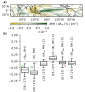
\includegraphics{sections/result_3/figures/rh_map.pdf}
    \caption{Relative humidity at 500 hPa, RH, 
    regressed onto mean area of heavy precipitation features, $A_m$, 
    in interannual variability (a). 
    Boxplots of correlations and partial correlations outside the influence of the total area \add[\firstAuthorEdit]{coverage} of heavy precipitation, 
    \change[\firstAuthorEdit]{$A_f$}{$C$}, of $RH$ and $A_m$, mean distance of heavy precipitation to 180$^\circ{}$E, \change[\firstAuthorEdit]{$C_z$}{$P_{z}$}, 
    and mean distance of heavy precipitation to the \add{geographic and hydrological} equator, \change[\firstAuthorEdit]{$C_m$}{$P_{eq}$ and $P_{heq}$} (b). 
    Star and diamond show results for observations and high-resolution GCM, respectively, shown in lighter colors if not statistically significant. 
    The numbers below the boxplots gives the fraction of models with statistically significant correlations.}
\label{radiation_obsMAP_BOX_RH}
\end{figure}

\begin{figure}
    \centering
    \includegraphics{sections/result_3/figures/lcf_map.pdf}
    \caption{Same as Figure 12, 
    but with the low cloud fraction, LCF, 
    and low cloud fraction in regions of descent, LCF$_d$, 
    as response variable.}
\label{radiation_obsMAP_BOX_LCF}
\end{figure}
\clearpage

Consistent with the results from the previous section, 
models with larger increases in large-scale clustering under warming 
tend to have changes in relative humidity and clouds consistent with an El Ni\~no-like shift in the tropical circulation. 
The regression patterns of RH and LCF onto changes in $A_m$ under warming across the CMIP6 ensemble 
(Figure S\change[\firstAuthorEdit]{10}{8}a-b) are similar to those for interannual variability presented above. 
However, in contrast to the case for interannual variability, changes in \change[\firstAuthorEdit]{large-scale clustering}{overall clustering according to $A_m$} with warming 
have little connection to changes in tropical-mean mean RH or low-cloud fraction in regions of descent, LCF$_d$, across the CMIP6 ensemble (Figure \ref{radiation_SCATTER}a, b). 
Given this, it is perhaps not surprising that there is no correlation between the increase in $A_m$ within a model under warming and the model's ECS (Figure \ref{radiation_SCATTER}c). 
Here we take ECS from the supplementary material of \citet{Zelinka2020} and \citet{hausfather2022}.

The results therefore indicate that changes in \change[\firstAuthorEdit]{large-scale clustering}{a general clustering of heavy precipitation features, $A_m$,} under warming 
do not strongly affect radiative feedbacks, despite indications from observations that more clustered states \add[\firstAuthorEdit]{in this way} are drier with more low-clouds in regions of large-scale descent. 
One reason for this result appears to be the different ways in which large-scale clustering \add[\firstAuthorEdit]{of heavy rainfall} can manifest at different timescales. 
In interannual variability, increases in \add{heavy precipitation} clustering are associated with increases in the 
\change[\firstAuthorEdit]{
fractional area 
}{
total area coverage
}
of heavy precipitation, defined here by \change[\firstAuthorEdit]{$A_f$}{$C$}. 
Under climate change, increases in \change[\firstAuthorEdit]{$A_f$}{$C$} in one month must be balanced by decreases in another month 
such that the overall average must remain constant. 
When the effects of changes in 
\change[\firstAuthorEdit]{
area fraction 
}{
total area coverage
}
are removed, the observed relationship to RH becomes weak. 
However, this explanation is not the whole story, as many of the models do exhibit changes in RH associated with increased clustering 
independent of changes in the 
\change[\firstAuthorEdit]{
area fraction 
}{
total area coverage
}
of heavy precipitation. Even among this subset of models, however, 
future increases in $A_m$ are not a good predictor of future changes in clouds or relative humidity. 
This suggests that caution should be used in extrapolating relationships---either observed or simulated---between large-scale clustering 
and other properties of the climate in internal variability to those for climate change.

Finally, we note that there does exist a relationship between a tropical-mean drying \add[\firstAuthorEdit]{and LCF in some key subsidence regions} with
the proximity of heavy rainfall to the \add{geographic and hydrological equator (Figure S2 and S8g-h in supporting information)}. 
Under warming, variations in the meridional contraction of heavy rainfall, 
as measured by the mean distance of heavily precipitating girdpoints to the equator \change[\firstAuthorEdit]{$C_m$}{$P_{eq}$}, 
explain about 45 percent of the variance in tropical-mean drying 
(Figure \ref{radiation_warming_MAP} and Figure \ref{radiation_warming_SCATTER}). 
This relationship is consistent with the sign of the relationship between RH and \change[\firstAuthorEdit]{$C_m$}{$P_{eq}$} 
in interannual variability in a subset of CMIP6 models (Figure \ref{radiation_obsMAP_BOX_RH}b). 
This result potentially highlights the importance of ITCZ narrowing as a specific manifestation of large-scale clustering 
that appears to be important for setting the tropical-mean relative humidity. 
However, we note that most of the spread in projected drying is due to the result of four models with dramatically different drying trends\change[\firstAuthorEdit]{, and t}{.} \add[\firstAuthorEdit]{When
these 4 models are removed from the ensemble, the correlation is no longer present. 
Thus further work is required to confirm if this relationship is robust and physical.
}

\clearpage
\begin{figure}
    \centering
    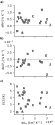
\includegraphics{sections/result_3/figures/rh_lcf_ecs.pdf}
    \caption{Scatter plot of change in $A_m$ between historical period and SSP585 period per Kelvin tropical warming and associated tropical-mean change in 
    500 hPa relative humidity, RH, (a), 
    low cloud fraction in regions of descent, LCF$_d$ (b), 
    and equilibrium climate sensitivity (ECS) in the CMIP6 ensemble (c). 
    Models are as given in the legend in Figure 4.}
\label{radiation_SCATTER}
\end{figure}

\clearpage
\begin{figure}
    \centering
    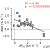
\includegraphics{sections/result_3/figures/rh_cm.pdf}
    \caption{Scatter plot of change in mean distance of heavy precipitation to the \add[\firstAuthorEdit]{geographic} equator, \change[\firstAuthorEdit]{$C_m$}{$P_{eq}$}, 
    between historical period and SSP585 period per Kelvin tropical warming and associated tropical-mean change in 500hPa relative humidity, RH.
    Models are as given in the legend in Figure 4.
    \remove[\firstAuthorEdit]{The values are plotted as anomalies from the ensemble mean and}
    }
\label{radiation_warming_SCATTER}
\end{figure}

\begin{figure}
    \centering
    \includegraphics{sections/result_3/figures/cm_rh_map.pdf}
    \caption{Change in relative humidity at 500 hPa, RH, 
    regressed onto changes in mean distance of heavy precipitation to the \add[\firstAuthorEdit]{geographic} equator, \change[\firstAuthorEdit]{$C_m$}{$P_{eq}$}, 
    between the historical and SSP585 periods per Kelvin warming.}
\label{radiation_warming_MAP}
\end{figure}



